\documentclass[12pt]{article}
\usepackage[hmargin=1.4in,vmargin=1.4in]{geometry}
\bibliographystyle{ecta}
\usepackage[pdftex]{graphicx}
\usepackage[outdir=../output/figures/]{epstopdf}
\usepackage{tikz}
\usepackage{subfigure}
\usepackage{amsthm, amsmath, amsfonts}
\usepackage{xcolor}
\usepackage{tcolorbox}
\usepackage{enumerate}
\usepackage[onehalfspacing]{setspace}
\usepackage{multirow}
\usepackage{cancel}
\usepackage{booktabs}
\usepackage{epstopdf}
\usepackage{bm}
\usepackage{apptools}
\usepackage[multiple]{footmisc}
\usepackage[hidelinks,hyperfootnotes=false]{hyperref}
\usepackage{fancyhdr}
\usepackage{footnote}
\usepackage{floatrow}
\usepackage{array}
\usepackage{float}
\usepackage{hyperref}
\usepackage{xr}
\usepackage{pdflscape}
\usepackage{caption}
\allowdisplaybreaks
\newcommand{\tunderbrace}[1]{\underbrace{\textstyle#1}}
\newcommand{\toverbrace}[1]{\overbrace{\textstyle#1}}
\makeatletter
\newcommand{\vast}{\bBigg@{3}}
\newcommand{\Vast}{\bBigg@{4}}
\makeatother
\makeatletter\let\expandableinput\@@input\makeatother
\newcolumntype{L}[1]{>{\raggedright\arraybackslash}m{#1}}
\newcolumntype{C}[1]{>{\centering\arraybackslash}m{#1}}


\begin{document}
\section{Numerical solution: main text}

\begin{table}[H]
\centering
\bgroup
\def\arraystretch{1.25}
\begin{tabular}{clclcc} \hline
& Description & Value & Moment & Target & Model \\ 
\hline 
$\sigma^z$ & std. dev. prod. & 0.55\% & $\sigma(\Delta\log c)$ & 0.5\% & 0.6\% \\ 
$\chi^x$ & capital adj. cost & 3.5     & $\sigma(\Delta\log x)$ & 2.1\% & 2.0\% \\ 
$\beta$ & discount factor & 0.98     & $4r_{+1}$ & 1.3\% & 1.5\% \\ 
$\gamma^b$ & RRA $b$ & 25.5     & $4[r^e_{+1}-r_{+1}]$ & 7.3\% & 7.0\% \\ 
$\sigma^p$ & std. dev. log dis. prob. &   0.47  & $\sigma(4\mathbb{E}r_{+1})$ & 2.2\% & 2.2\% \\ 
$\rho^p$ & persist. log dis. prob. & 0.8     & $\rho(\mathbb{E}r_{+1})$ & 0.79     & 0.75     \\ 
$\gamma^a$ & RRA $a$ & 10  & $q k^a/a^a$ & 2.0     & 2.3     \\ 
$\underline{k}$ & lower bound $k^i$ & 10     & $q k^c/a^c$ & 1.1     & 0.9     \\ 
$\xi\bar{s}^a$ & newborn endowment $a$ & 0\% & $\lambda^aa^a/\sum_i\lambda^ia^i$ & 18\% & 21\% \\ 
$\xi\bar{s}^c$ & newborn endowment $c$ & -0.25\% & $\lambda^ca^c/\sum_i\lambda^ia^i$ & 23\% & 23\% \\ 
$b^g$ & real value govt. bonds &   -2.7  & $-\sum_i\lambda^ib^i/\sum_i\lambda^ia^i$ & -10\% & -10\% \\ 
\hline 
\multicolumn{6}{@{}l}{\scriptsize Disutility parameters $\bar{\nu}^i$ set to $(  0.64,   2.89,   0.43)$ to jointly match average labor and steady state labor income shares.} \\ 
\hline 

\end{tabular}
\egroup
\renewcommand\thetable{V}
\caption{targeted moments and calibrated parameters}
\label{tab:cal}
\end{table}

\pagebreak

\begin{table}[H]
\centering
\bgroup
\def\arraystretch{1.25}
\begin{tabular}{lC{17mm}C{17mm}C{17mm}} \hline
Moment & Data & Model \\ 
\hline 
$\sigma(\Delta\log y)$ & $   0.8\%$ & $   0.9\%$ \\ 
$\sigma(\Delta\log \ell)$ & $   0.8\%$ & $   0.8\%$ \\ 
$\sigma(d/p)$ & $   0.2\%$ & $   0.2\%$ \\ 
\hline 
$\sum_i\lambda^impr^i$ & $\approx   0.2$ & $   0.3$ \\ 
$mpr^a$ & & $   1.9$ \\ 
$mpr^b$ & & $   0.7$ \\ 
$mpr^c$ & & $   0.0$ \\ 
\hline 
$\sum_i\lambda^impc^i$ & $\approx   0.2$ & $  0.02$ \\ 
$mpc^a$ & & $  0.02$ \\ 
$mpc^b$ & & $  0.02$ \\ 
$mpc^c$ & & $  0.02$ \\ 
\hline 

\end{tabular}
\egroup
\renewcommand\thetable{VI}
\caption{untargeted macro and micro moments}
\label{tab:untargeted}
\end{table}

\vspace{40pt}

\begin{figure}[H]
\centering
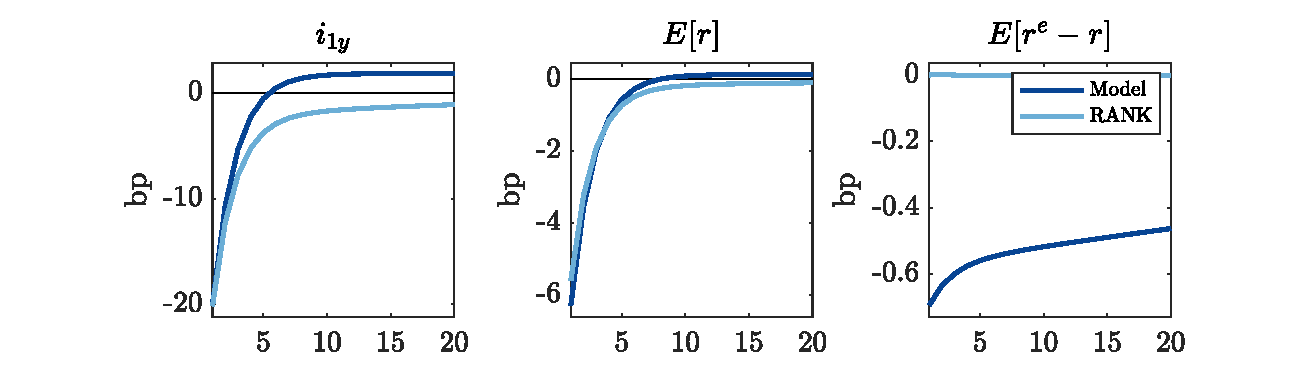
\includegraphics[width=\textwidth,clip=true,trim=0 0 0 0]{../output/figures/monetary_fig_split1}
\renewcommand\thefigure{2}
\caption{expected returns after negative monetary policy shock}
\end{figure}

\pagebreak

\begin{figure}[H]
\centering
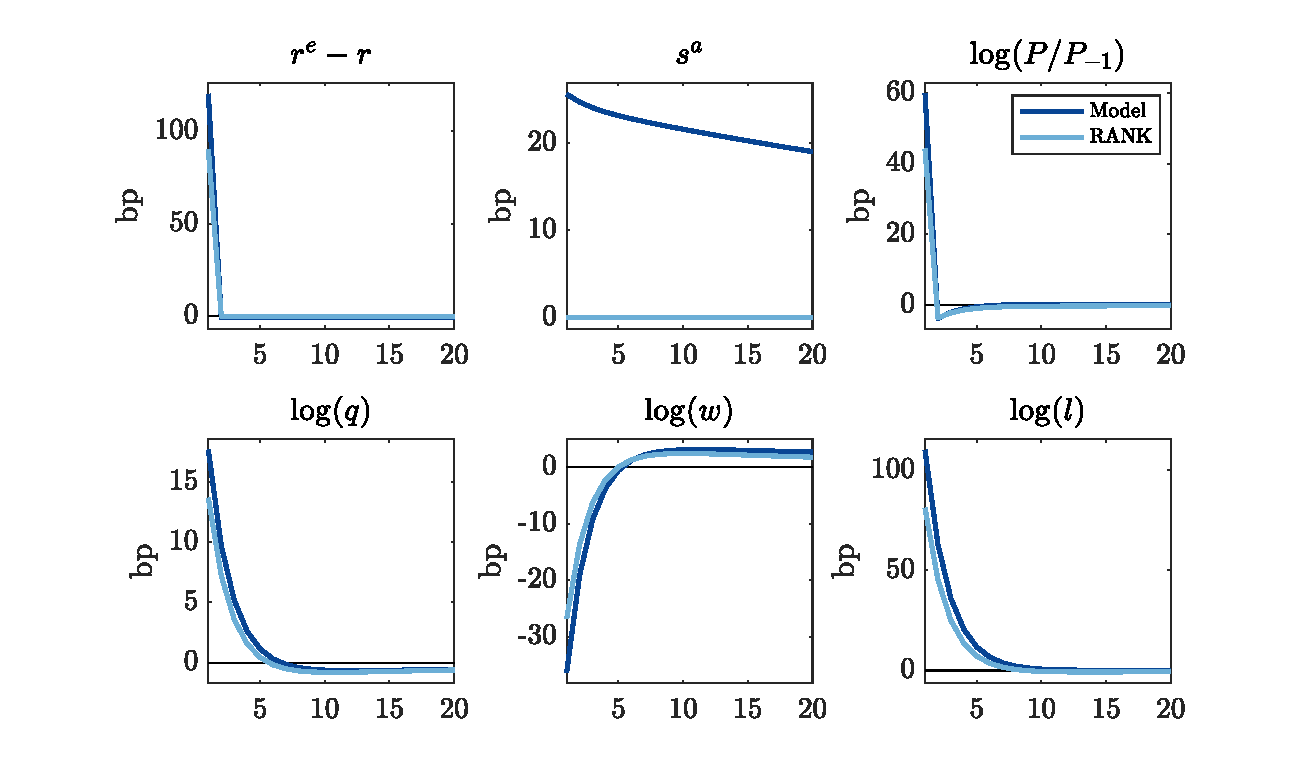
\includegraphics[width=\textwidth,clip=true,trim=0 20 0 10]{../output/figures/monetary_fig_split2}
\renewcommand\thefigure{3}
\caption{redistribution after negative monetary policy shock}
\end{figure}

\vspace{40pt}

\begin{figure}[H]
\centering
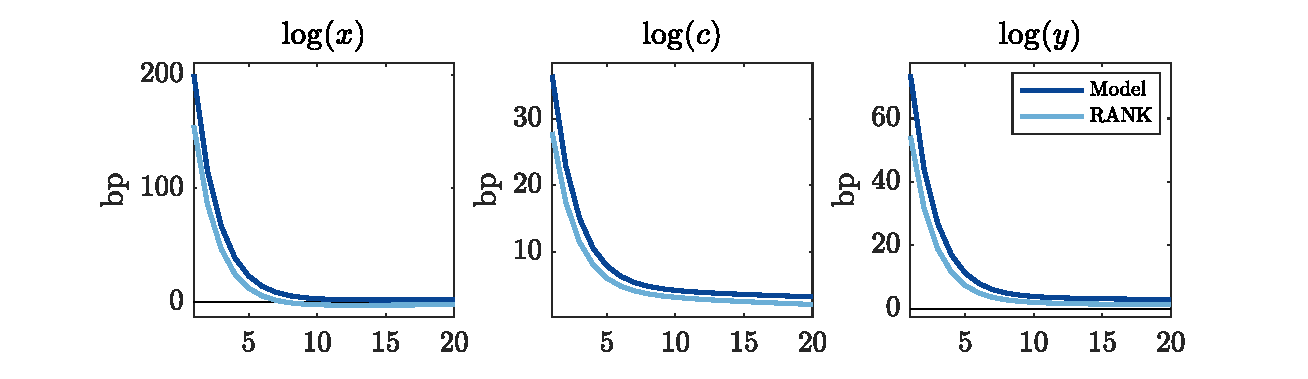
\includegraphics[width=\textwidth,clip=true,trim=0 0 0 0]{../output/figures/monetary_fig_split3}
\renewcommand\thefigure{4}
\caption{quantities after negative monetary policy shock}
\end{figure}

\pagebreak

\begin{table}[H]
\centering
\bgroup
\def\arraystretch{1.25}
\begin{tabular}{lC{35mm}C{18mm}C{17mm}} \hline
\% Real stock return & Data [90\% CI] & Model & RANK \\ 
\hline 
Dividend growth news & 33\% [-13\%,71\%] &     52\% &     65\% \\ 
$-$ Future real rate news & 8\% [-6\%,21\%] &     16\% &     35\% \\ 
$-$ Future excess return news & 59\% [19\%,108\%] &     32\% &      0\% \\ 
\hline 

\end{tabular}
\egroup
\renewcommand\thetable{VII}
\caption{Campbell-Shiller decomposition of stock market return after monetary shock}
\end{table}

\vspace{20pt}

\begin{table}[H]
\centering
\bgroup
\def\arraystretch{1.25}
\begin{tabular}{lC{18mm}C{18mm}C{25mm}} \hline
  &  Model & RANK & Model/RANK \\ 
\hline 
 $\Delta\log(y)$ & $     74 bp$ & $     54 bp$ & $    1.4$ \\ 
 $\Delta\log(c)$ & $     37 bp$ & $     28 bp$ & $    1.3$ \\ 
 $\Delta\log(x)$ & $    200 bp$ & $    155 bp$ & $    1.3$ \\ 
\hline 

\end{tabular}
\egroup
\caption*{Real effects of monetary shock}
\end{table}

\pagebreak

\begin{table}[H]
\centering
\bgroup
\def\arraystretch{1.25}
\begin{tabular}{lC{15mm}C{15mm}C{15mm}} \hline 
\expandableinput ../output/tables/decomp_tab_1.tex
\end{tabular}
\egroup
\renewcommand\thetable{VIII}
\caption{decomposing capital accumulation on impact of shock}
\end{table}

\vspace{20pt}

\begin{table}[H]
\centering
\bgroup
\def\arraystretch{1.25}
\begin{tabular}{lC{13mm}C{13mm}C{13mm}C{14mm}} \hline 
\expandableinput ../output/tables/decomp_tab_2.tex
\end{tabular}
\egroup
\renewcommand\thetable{IX}
\caption{decomposing wealth redistribution to $a$ households on impact of shock}
\end{table}

\pagebreak

\section{Numerical solution: appendix}


\begin{figure}[H]
\centering
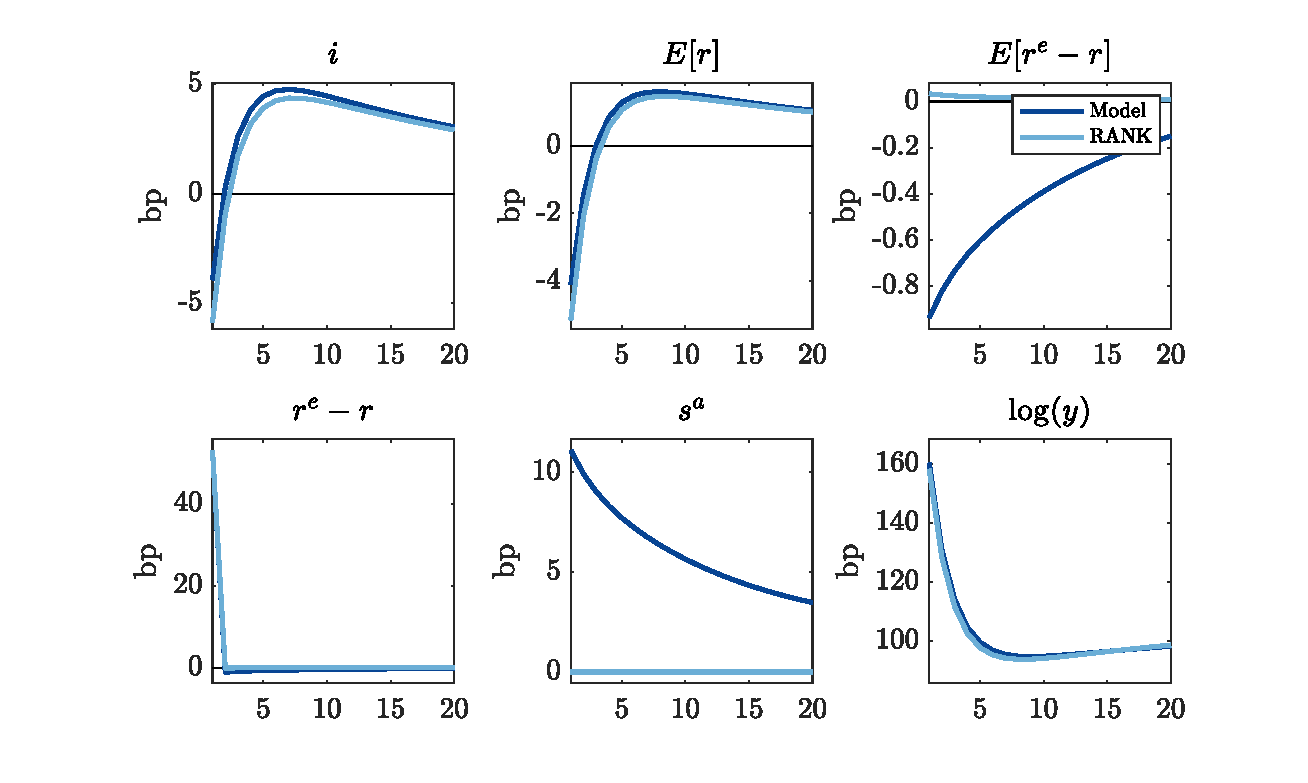
\includegraphics[width=\textwidth,clip=true,trim=0 20 0 10]{../output/figures/TFP_compact_fig}
\renewcommand\thefigure{A.2}
\caption{impulse responses to positive productivity shock}
\end{figure} 


\begin{figure}[H]
\centering
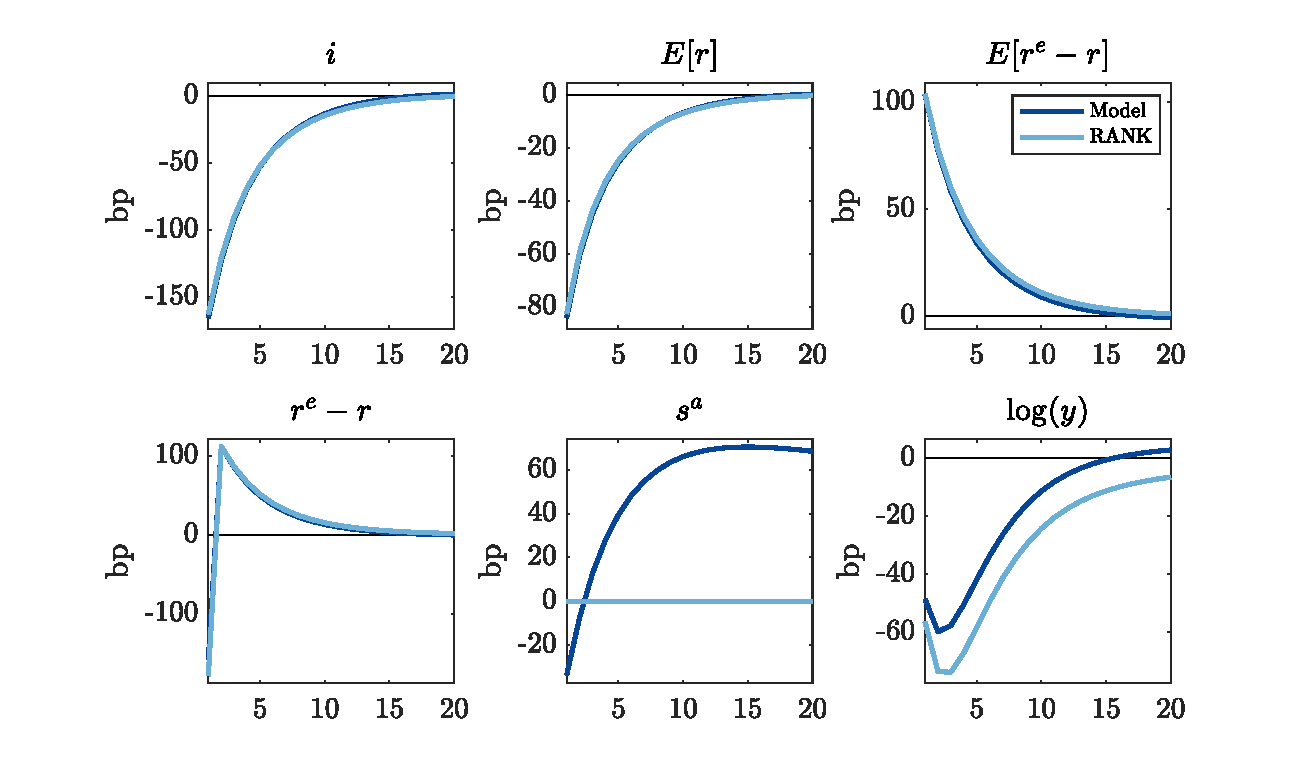
\includegraphics[width=\textwidth,clip=true,trim=0 20 0 10]{../output/figures/dis_compact_fig}
\renewcommand\thefigure{A.3}
\caption{impulse responses to positive disaster probability shock}
\end{figure} 

\pagebreak

\begin{table}[H]
\centering
\bgroup
\def\arraystretch{1.25}
\begin{tabular}{clclcc} \hline
& Description & Value & Moment & Target & Model \\ 
\hline 
$\sigma^z$ & std. dev. prod. & 0.55\% & $\sigma(\Delta\log c)$ & 0.5\% & 0.6\% \\ 
$\chi^x$ & capital adj. cost & 3.5     & $\sigma(\Delta\log x)$ & 2.1\% & 2.0\% \\ 
$\beta$ & discount factor & 0.984     & $4r_{+1}$ & 1.3\% & 1.1\% \\ 
$\gamma^b$ & RRA $b$ & 21     & $4[r^e_{+1}-r_{+1}]$ & 7.3\% & 7.3\% \\ 
$\sigma^p$ & std. dev. log dis. prob. &   0.47  & $\sigma(4\mathbb{E}r_{+1})$ & 2.2\% & 2.2\% \\ 
$\rho^p$ & persist. log dis. prob. & 0.8     & $\rho(\mathbb{E}r_{+1})$ & 0.79     & 0.74     \\ 
$\gamma^a$ & RRA $a$ & 2.5  & $q k^a/a^a$ & 4.4     & 4.8     \\ 
$\underline{k}$ & lower bound $k^i$ & 10     & $q k^c/a^c$ & 1.1     & 1.0     \\ 
$\xi\bar{s}^a$ & newborn endowment $a$ & 0\% & $\lambda^aa^a/\sum_i\lambda^ia^i$ & 2\% & 3\% \\ 
$\xi\bar{s}^c$ & newborn endowment $c$ & 0.9\% & $\lambda^ca^c/\sum_i\lambda^ia^i$ & 23\% & 24\% \\ 
$b^g$ & real value govt. bonds &   -2.7  & $-\sum_i\lambda^ib^i/\sum_i\lambda^ia^i$ & -10\% & -10\% \\ 
\hline 
\multicolumn{6}{@{}l}{\scriptsize Disutility parameters $\bar{\nu}^i$ set to $(  0.00,   2.47,   0.44)$ to jointly match average labor and steady state labor income shares.} \\ 
\hline 

\end{tabular}
\egroup
\renewcommand\thetable{A.IV}
\caption{targeted moments and calibrated parameters, alternative calibration}
\end{table}

\begin{figure}[H]
\centering
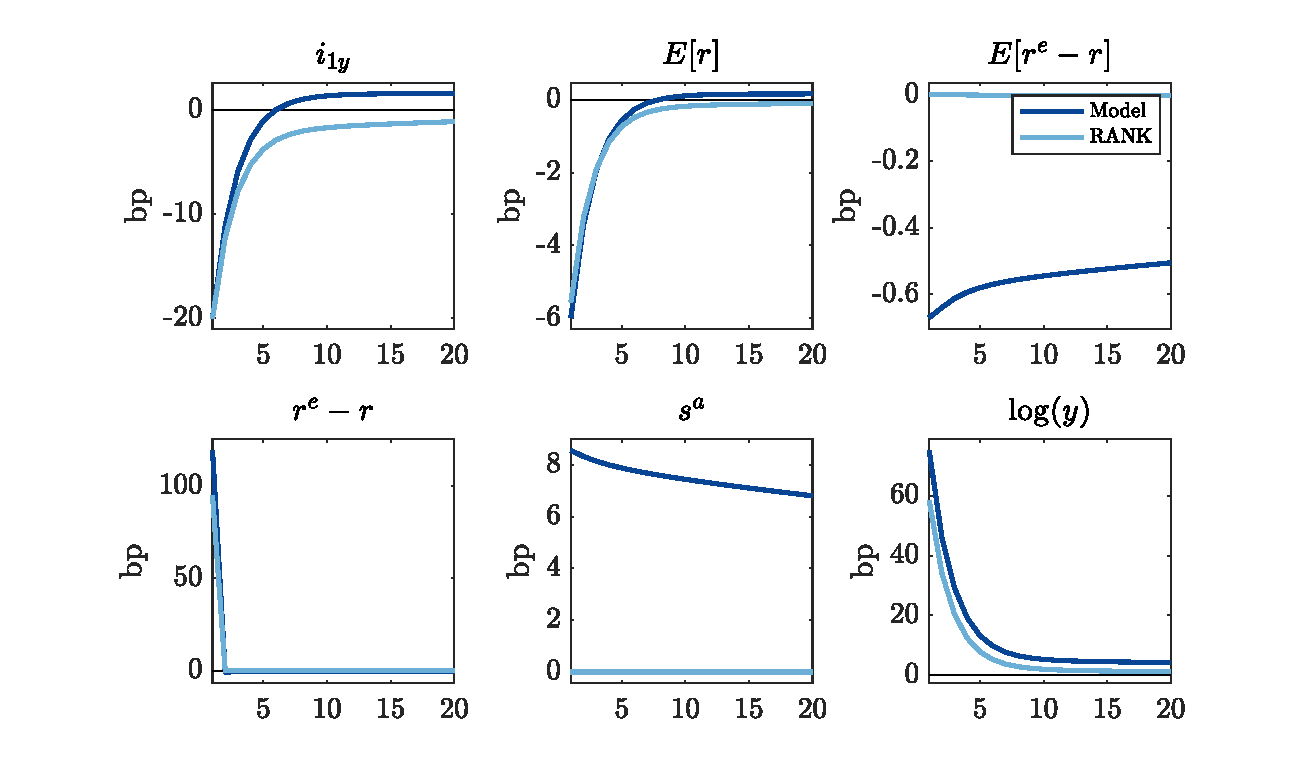
\includegraphics[width=\textwidth,clip=true,trim=0 20 0 10]{../output/figures/interm_compact_fig}
\renewcommand\thefigure{A.5}
\caption{quantities after negative monetary policy shock, alternative calibration}
\end{figure}

\vspace{20pt}

\begin{table}[H]
\centering
\bgroup
\def\arraystretch{1.25}
\begin{tabular}{lC{35mm}C{18mm}C{17mm}} \hline
\% Real stock return & Data [90\% CI] & Model & RANK \\ 
\hline 
Dividend growth news & 33\% [-13\%,71\%] &     50\% &     65\% \\ 
$-$ Future real rate news & 8\% [-6\%,21\%] &     13\% &     35\% \\ 
$-$ Future excess return news & 59\% [19\%,108\%] &     37\% &      0\% \\ 
\hline 

\end{tabular}
\egroup
\renewcommand\thetable{A.V}
\caption{decomposition after monetary shock, alternative calibration}
\end{table}

\vspace{10pt}

\begin{table}[H]
\centering
\bgroup
\def\arraystretch{1.25}
\begin{tabular}{lC{18mm}C{18mm}C{25mm}} \hline
  &  Model & RANK & Model/RANK \\ 
\hline 
 $\Delta\log(y)$ & $     75 bp$ & $     58 bp$ & $    1.3 $ \\ 
 $\Delta\log(c)$ & $     37 bp$ & $     29 bp$ & $    1.3 $ \\ 
 $\Delta\log(x)$ & $    201 bp$ & $    156 bp$ & $    1.3 $ \\ 
\hline 

\end{tabular}
\egroup
\caption*{Real effects of monetary shock}
\end{table}

%%%%%%%%%%%%%%%%%%%%%%%%%%%%%%%%%%%%%%%%%%%%%%%%%

\begin{table}[H]
\centering
\bgroup
\def\arraystretch{1.25}
\begin{tabular}{clclcc} \hline
& Description & Value & Moment & Target & Model \\ 
\hline 
$\sigma^z$ & std. dev. prod. & 0.55\% & $\sigma(\Delta\log c)$ & 0.5\% & 0.5\% \\ 
$\chi^x$ & capital adj. cost & 3.5     & $\sigma(\Delta\log x)$ & 2.1\% & 2.1\% \\ 
$\beta$ & discount factor & 0.98     & $4r_{+1}$ & 1.3\% & 1.4\% \\ 
$\gamma^a = \gamma^b = \gamma^c$ & RRA & 11     & $4[r^e_{+1}-r_{+1}]$ & 7.3\% & 7.4\% \\ 
$\sigma^p$ & std. dev. log dis. prob. &   1.20  & $\sigma(4\mathbb{E}r_{+1})$ & 2.2\% & 2.2\% \\ 
$\rho^p$ & persist. log dis. prob. & 0.8     & $\rho(\mathbb{E}r_{+1})$ & 0.79     & 0.70     \\ 
$\eta^b$ & idio. risk $b$ & 0.001  & $q k^a/a^a$ & 2.0     & 2.5     \\ 
$\underline{k}$ & lower bound $k^i$ & 10     & $q k^c/a^c$ & 1.1     & 0.9     \\ 
$\xi\bar{s}^a$ & newborn endowment $a$ & -0.02\% & $\lambda^aa^a/\sum_i\lambda^ia^i$ & 18\% & 22\% \\ 
$\xi\bar{s}^c$ & newborn endowment $c$ & -0.15\% & $\lambda^ca^c/\sum_i\lambda^ia^i$ & 23\% & 24\% \\ 
$b^g$ & real value govt. bonds &   -2.6  & $-\sum_i\lambda^ib^i/\sum_i\lambda^ia^i$ & -10\% & -10\% \\ 
\hline 
\multicolumn{6}{@{}l}{\scriptsize Disutility parameters $\bar{\nu}^i$ set to $(  0.64,   2.89,   0.43)$ to jointly match average labor and steady state labor income shares.} \\ 
\hline 

\end{tabular}
\egroup
\renewcommand\thetable{A.VI}
\caption{targeted moments and calibrated parameters, idiosyncratic risk}
\end{table}

\begin{figure}[H]
\centering
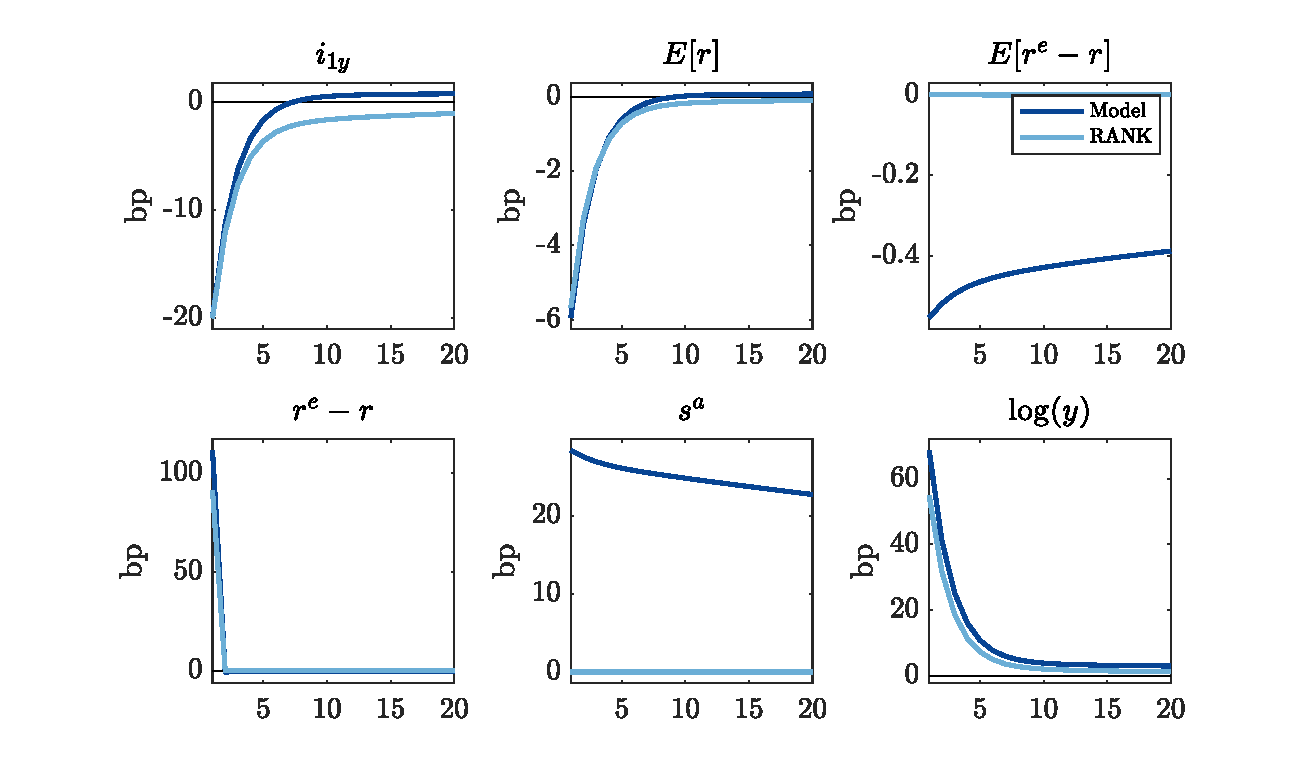
\includegraphics[width=\textwidth,clip=true,trim=0 20 0 10]{../output/figures/idio_compact_fig}
\renewcommand\thefigure{A.6}
\caption{responses to negative monetary policy shock, idiosyncratic risk}
\end{figure}

\vspace{20pt}

\begin{table}[H]
\centering
\bgroup
\def\arraystretch{1.25}
\begin{tabular}{lC{35mm}C{18mm}C{17mm}} \hline
\% Real stock return & Data [90\% CI] & Model & RANK \\ 
\hline 
Dividend growth news & 33\% [-13\%,71\%] &     51\% &     65\% \\ 
$-$ Future real rate news & 8\% [-6\%,21\%] &     20\% &     35\% \\ 
$-$ Future excess return news & 59\% [19\%,108\%] &     28\% &      1\% \\ 
\hline 

\end{tabular}
\egroup
\renewcommand\thetable{A.VII}
\caption{decomposition after monetary shock, idiosyncratic risk}
\end{table}

\vspace{10pt}

\begin{table}[H]
\centering
\bgroup
\def\arraystretch{1.25}
\begin{tabular}{lC{18mm}C{18mm}C{25mm}} \hline
  &  Model & RANK & Model/RANK \\ 
\hline 
 $\Delta\log(y)$ & $     69 bp$ & $     55 bp$ & $    1.3$ \\ 
 $\Delta\log(c)$ & $     33 bp$ & $     28 bp$ & $    1.2$ \\ 
 $\Delta\log(x)$ & $    190 bp$ & $    155 bp$ & $    1.2$ \\ 
\hline 

\end{tabular}
\egroup
\caption*{Real effects of monetary shock}
\end{table}

\end{document}


